\documentclass[tikz]{article}

% Packages
\usepackage[utf8]{inputenc} % Core latex bundle 
\usepackage[a4paper, total={6in, 9in}]{geometry} % Customize document dimensions and formats
\usepackage{changepage} % Customize page layout in middle of document
\usepackage[table]{xcolor} % Add color to tables
\usepackage{standalone} % Add figures and tables from other files
\usepackage{import} % Import glossary
\usepackage{graphics} % General color and formats
\usepackage{url} % URL formatting
\usepackage{breakurl} % URL formatting
\usepackage{enumitem} % Format list spacing 
\usepackage[hang]{footmisc} % Footnote margins
\usepackage{hyperref} % References
\usepackage{mathtools} % Useful tools for mathematical typesetting and replaces amsmath
\usepackage{amssymb,bm} % Math symbols
\usepackage{svg} % SVG
\usepackage{tikz} % Making charts
\usepackage{array,boldline,multirow,float,booktabs} % Added to make tables
\usepackage{stackengine} % Customize row heights
\usepackage{hhline} % Add double lines to table
\usepackage{multicol} % Two column lists
\usepackage{nicematrix} % Put table lines after color
\usepackage{wrapfig} % Wrap figures in text
\usepackage{tocloft,titletoc} % TOC package
\usepackage{titlesec} % Section spacing

% Paper formatting
\newlength\LabelWidth
\setlength\parindent{0pt}
\setlength{\parskip}{1em}

% Section spacing
\titlespacing*{\section}
  {0pt}{0.6\baselineskip}{0.6\baselineskip} % Modify section spacing - first \baselineskip is spacing before, second is spacing after the section
\titlespacing*{\subsection}
  {0pt}{0.6\baselineskip}{0.6\baselineskip} % Modify subsection spacing 
\titlespacing*{\subsubsection}
  {0pt}{0.6\baselineskip}{0.6\baselineskip} % Modify subsubsection spacing

% String formats
\newcommand{\code}[1]{\texttt{#1}}
\newcommand{\term}[1]{\textsl{#1}}

% Paper margins
\def\changemargin#1#2{\list{}{\rightmargin#2\leftmargin#1}\item[]}
\let\endchangemargin=\endlist

% Table of contents
\renewcommand{\contentsname}{Table of Contents}
\renewcommand{\cfttoctitlefont}{\Large\bfseries} % TOC title size
\renewcommand{\cftsecleader}{\cftdotfill{\cftdotsep}} % Add dots in TOC to sections
\renewcommand{\cftsecpagefont}{} % Remove \bfseries from section titles' page in TOC

% Section
\renewcommand*{\cftsecnumwidth}{2em} % Increase space section from numbers on left
% \setlength{\cftbeforesecskip}{3pt} % Messes with section TOC length

% Subsection
\cftsetindents{subsection}{1em}{3em} % space between numbers and toc subsections
\setlength{\cftsubsecindent}{2.5em} % subsection number spacing from left
\setlength{\cftbeforesubsecskip}{3pt} % Messes with subsection TOC length was 3pt

% Subsubsection
\cftsetindents{subsubsection}{1em}{4em} % space between numbers and toc subsubsections
\setlength{\cftsubsubsecindent}{5.5em} % subsubsection number spacing from leftindent
\setlength{\cftbeforesubsubsecskip}{3pt} % Messes with subsubsection TOC length was 3pt

% extra paragraph & sub paragraph section
\setcounter{secnumdepth}{5}
\setcounter{tocdepth}{5}

% pagraph
\cftsetindents{paragraph}{1em}{5em} % space between numbers and toc paragraph
\setlength{\cftparaindent}{9.5em} % paragraph number spacing from leftindent
\setlength{\cftbeforeparaskip}{3pt} % Messes with paragraph TOC length was 3pt

% indent after paragraph section
\titleformat{\paragraph}
{\normalfont\normalsize\bfseries}{\theparagraph}{1em}{}
\titlespacing*{\paragraph}
{0pt}{3.25ex plus 1ex minus .2ex}{1.5ex plus .2ex}

% sub paragraph
\cftsetindents{subparagraph}{1em}{5em} % space between numbers and toc paragraph
\setlength{\cftsubparaindent}{14.5em} % paragraph number spacing from leftindent
\setlength{\cftbeforesubparaskip}{3pt} % Messes with paragraph TOC length was 3pt

% indent after subparagraph section
\titleformat{\subparagraph}
{\normalfont\normalsize\bfseries}{\thesubparagraph}{1em}{}
\titlespacing*{\subparagraph}
{0pt}{3.25ex plus 1ex minus .2ex}{1.5ex plus .2ex}


% Abstract
% Make abstract justified
\makeatletter
\newcommand{\justified}{
  \rightskip\z@skip
  \leftskip\z@skip}
\makeatother

% Format and size abstract
\makeatletter
\renewenvironment{abstract}{
    \if@twocolumn
      \section*{\abstractname}
    \else 
      \begin{center}
        {\bfseries \large\abstractname\vspace{\z@}} % Bolds abstract name
      \end{center}
      \quotation
    \fi}
    {\if@twocolumn\else\endquotation\fi}
\makeatother

% Delimiters
\DeclarePairedDelimiter\floor{\lfloor}{\rfloor} % Define paired delimiter for floor function
\DeclarePairedDelimiter{\ceil}{\lceil}{\rceil} % Define paired delimiter for ceiling function

% Hyperlinks
\hypersetup{
    colorlinks=true,
    linkcolor=black,
    filecolor=blue,
    urlcolor=black,
}
\urlstyle{same}

% Footnotes
\newcommand{\fref}[1]{\footnote{\href{http://#1}{#1}}}
\setlength{\footnotemargin}{8mm} % Spacing between footnote number and body

% Include tables
\makeatletter
\newcommand{\includetable}[1]{%
  \@ifundefined{tablepath}{%
    \InputIfFileExists{#1}{}{}%
  }{%
    \InputIfFileExists{\tablepath/#1}{}{\InputIfFileExists{#1}{}{}}%
  }
}
\makeatother  

% Table formatting commands
\newcolumntype{Q}{ >{\centering\arraybackslash} m{2.4cm} } % (Figure 5 and 11 - col width)
\newcolumntype{S}{ >{\centering\arraybackslash} m{5.27cm} } % (Figure 12 - col width double)
\newcommand\xrowht[2][0]{\addstackgap[.5\dimexpr#2\relax]{\vphantom{#1}}} % Set row height for tables
\newcommand{\rowh}[1]{\xrowht{40pt}} % Command to set row height for cell with 3 rows
\newcommand{\rowm}[1]{\xrowht{26.667pt}} % Command to set row height for cell with 2 rows
\newcommand{\rows}[1]{\xrowht{13.333pt}} % Command to set row height for cell with 1 rows

% Bean symbols
\newcommand{\BeanCover}{\includesvg[scale=2.2]{./logos/black-bean.svg}} % Logo on cover page
\newcommand{\Bean}{\includesvg[scale=0.23]{./logos/bean.svg}} % Bean used throughout the paper in text form
\newcommand{\bean}{\includesvg[scale=0.17]{./logos/microbean-wide.svg}} % Bean used in formulas - micro bean wide

% \newcommand{\Root}{\includesvg[scale=0.05]{./logos/root.svg}} % root logo
\newcommand{\Root}{\includesvg[scale=0.06]{./logos/root-tiny.svg}} % root logo
\newcommand{\RootCover}{\includesvg[scale=1]{./logos/root.svg}} % Logo on cover page

\newcommand{\tinybean}{\includesvg[scale=0.13]{./logos/microbean-wide.svg}} % Bean used in formulas - micro bean wide

\newcommand{\lambdabean}{\includesvg[scale=0.17]{./logos/microbean.svg}} % Bean used in formulas for lambda superscript - micro bean

% List Key
\SetEnumitemKey{midsep}{topsep=0pt, itemsep=3pt} % Itemize key

% File paths
\newcommand{\tablepath}{figures} % Tables file path
\graphicspath{{figures/}} % Figures file path


%%%%%%%   Begin Document   %%%%%%%
\begin{document}
\pagenumbering{arabic} % Start page numbering style
\thispagestyle{empty} % Hide page numbering
\begin{titlepage}
    \begin{center}
        \vspace*{-0.1cm}
        \begin{changemargin}{-0.25cm}{-0.25cm}
        \centering % added to center title
        \textbf{\Large{Root: Fungibility for Beanstalk Silo Deposits}}
        \end{changemargin}
        \begin{center}
        \RootCover
        \end{center}
        \vspace{0.4cm}
        \large{Kokonut, Mistermanifold, Sarrdinero and Publius}
            
        \vspace{-0.25cm}
        \normalsize{roottoken@protonmail.com}
        
        \vspace{-0.25cm}
        \normalsize{\href{https://roottoken.org/}{roottoken.org}}
        
        \vspace{0.4cm}
        \footnotesize{Published:} \normalsize{November 16, 2022}
        
        \vspace{-0.25cm}
        \footnotesize{Modified:} \normalsize{December 4, 2022}
        
        \vspace{-0.25cm}
        \footnotesize{Whitepaper Version:} {\normalsize{1.0.2}}
        
        \vspace{-0.25cm}
        \footnotesize{Code Version:} \href{https://github.com/RootToken/Root}{\normalsize{1.0.1}}\footnote{\href{https://github.com/RootToken/Root}{github.com/RootToken/Root}}

        \vspace{0.1cm}
        \flushleft{\normalsize{\term{“Out of intense complexities, intense simplicities emerge.”}}}
        
        \normalsize{\hspace{2.5em}- Winston Churchill, The World Crisis}
        \vspace{0.4cm}
        \begin{abstract}
            \justified{\normalsize{\noindent Beanstalk\fref{bean.money/beanstalk.pdf} \term{Silo} \term{Deposits}\footnote{Any italicized terms not defined herein are defined by Beanstalk.} are not fungible. A fungible wrapper for \term{Silo} \term{Deposits} can create additional utility for Beans, particularly before a standard interface for other protocols to interact with \term{Silo} \term{Deposits} exists. Root is a fungible wrapper for Beanstalk \term{Silo} \term{Deposits} that implements the ERC-20 Standard. Any Ethereum account can \term{Mint} and \term{Redeem} Roots (\Root), the Root ERC-20 Standard token, for \term{Silo} \term{Deposits}. A decentralized autonomous organization (DAO) governed by \Root\ owners facilitates the coordination of Root upgrades and collective participation in Beanstalk governance.}}
        \end{abstract}
   \end{center}
\end{titlepage}

\newpage

% TOC formatting
% \addtocontents{toc}{\protect\enlargethispage{20mm}} % TOC margins
\thispagestyle{empty} % Hide TOC page numbering 
\addtocontents{toc}{\protect\thispagestyle{empty}} % Allow hiding both TOC page numbers

\cleardoublepage
\pagenumbering{gobble}
{\large\tableofcontents} % Compile TOC with large font
\cleardoublepage
\pagenumbering{arabic}

% \thispagestyle{empty} % Hide TOC page numbering
% \addtocontents{toc}{\protect\thispagestyle{empty}} % Allow hiding both TOC page numbers

\newpage
\setcounter{page}{3} % Begin page numbering

\section{Introduction}
Beanstalk is an Ethereum-native permissionless fiat stablecoin protocol. Beanstalk's credit  based stability model is a potential solution to the stablecoin carrying cost problem plaguing decentralized finance (DeFi). Whereas other stablecoin protocols rely on collateral to issue stablecoins, which creates centralization and carrying costs, Beanstalk uses infinitely scalable decentralized credit to create a permissionless stablecoin, Bean (\Bean), that has carrying costs competitive with off-chain fiat.

While Bean is an ERC-20 Standard token, in order to receive Beanstalk-native passive interest, Beans must be \term{Deposited} in the \term{Silo}, the Beanstalk DAO, directly or wrapped in whitelisted\fref{bean.money/beanstalk.pdf\#subsection.14.2} liquidity pool (LP) tokens. Beanstalk evaluates the flash-loan-resistant Bean-denominated-value (BDV) of each \term{Deposit}, at the time of \term{Deposit}. However, \term{Silo} \term{Deposits} have two qualities that make them non-fungible: the \term{Stalk} and \term{Seeds} per BDV of each \term{Deposit}. The non-fungibility of \term{Silo} \term{Deposits} appears necessary to Beanstalk's peg maintenance mechanism, but currently comes at the cost of composability. 

Composability is one of the core value propositions of blockchains. In order to facilitate composability, there are a variety of Ethereum token Standards that are widely adopted by various DeFi protocols. The ERC-20 Standard is the benchmark fungible token standard of the Ethereum network. Root is an Ethereum-native permissionless wrapper that implements the ERC-20 token Standard to create fungibility and composability for Beanstalk \term{Silo} \term{Deposits}.

\section{Previous Work}
Root uses the OpenZeppelin\fref{github.com/OpenZeppelin/openzeppelin-contracts-upgradeable} implementation of the ERC-20 Standard.

EIP-4626 formalized a Standard for token vaults, but only supports a single underlying ERC-20 Standard token. 

Root is implemented on top of Beanstalk. 

\section{Root}
Root is a permissionless fungible wrapper that enables collective farming for Beanstalk \term{Silo} \term{Deposits}. 

Any Ethereum account can \term{Mint} and \term{Redeem} \Root\ for Beanstalk \term{Silo} \term{Deposits} on the \term{Minting} \term{Whitelist} through Root at anytime. Anytime \Root\ are \term{Minted} or \term{Redeemed}, the BDV, \term{Stalk} and \term{Seeds} per \Root\ either remain the same or increase. 

All value in Root is owned pro rata by \Root. Any account can contribute to collective farming by calling the \code{earn}, \code{mow}, \code{updateBDV} and \code{updateBDVs} functions.

\subsection{Minting Whitelist}
Any ERC-20 Standard token that is on the Beanstalk \term{Deposit} \term{Whitelist} can be added to and removed from the \term{Minting} \term{Whitelist} via Root governance. 

Any Beanstalk \term{Silo} \term{Deposit} of a token on the \term{Minting} \term{Whitelist} can be used to \term{Mint} \Root.

\subsection{Mint}
Any account can \term{Mint} \Root\ at anytime by calling the \code{mint} function with (1) the minimum \Root\ to \term{Mint} ($\Root^{\text{min}}$), such that $\Root^{\text{min}} \in \{j \times 10^{-18} \mid j \in \mathbb{N}\}$, and (2) a list of Beanstalk \term{Silo} \term{Deposits} of tokens on the \term{Minting} \term{Whitelist} not currently owned by Root with cumulative BDV ($\Sigma l$), cumulative \term{Stalk} ($\Sigma k$), such that $\Sigma k \in \{j \times 10^{-10} \mid j \in \mathbb{N}\}$,  and cumulative \term{Seeds} ($\Sigma c$), such that $\Sigma l,\ \Sigma c \in \{j \times 10^{-6} \mid j \in \mathbb{N}\}$. If the total \Root\ supply ($\rho$) is 0, the \Root\ received upon \term{Minting} ($\Root^{+}$), such that $\rho ,\ \Root^{+} \in \{j \times 10^{-18} \mid j \in \mathbb{N}\}$, is $\Sigma k$ times $10^{8}$. Otherwise, the \Root\ received upon \term{Minting} is the maximum of (1) $\Root^{\text{min}}$ and (2) the minimum of the percentage change in the BDV, \term{Stalk} and \term{Seeds} of Root as a result of the \term{Mint}, times $\rho$. 

Therefore, we define $\Root^{+}$ for a given $\rho$, $\Root^{\text{min}}$, list of \term{Silo} \term{Deposits} with $\Sigma l$, $\Sigma k$ and $\Sigma c$, and Root total BDV ($L$), total \term{Stalk} ($K$), such that $K \in \{j \times 10^{-10} \mid j \in \mathbb{N}\}$, and total \term{Seeds} ($C$), such that $L,\ C \in \{j \times 10^{-6} \mid j \in \mathbb{N}\}$, as:
$$\Root^{+} = \begin{cases} \Sigma k \times 10^{8} & \text{if}\ \; \rho = 0 \vspace{.3cm} \\ 
\text{max}\left(\Root^{\text{min}},\ \text{min}\left(\frac{\Sigma l}{L},\ \frac{\Sigma k}{K},\ \frac{\Sigma c}{C}\right) \times \rho \right) & \text{else}\end{cases}$$

\begin{figure}[h!]
    \centering
    \hbox{\hspace{6em} 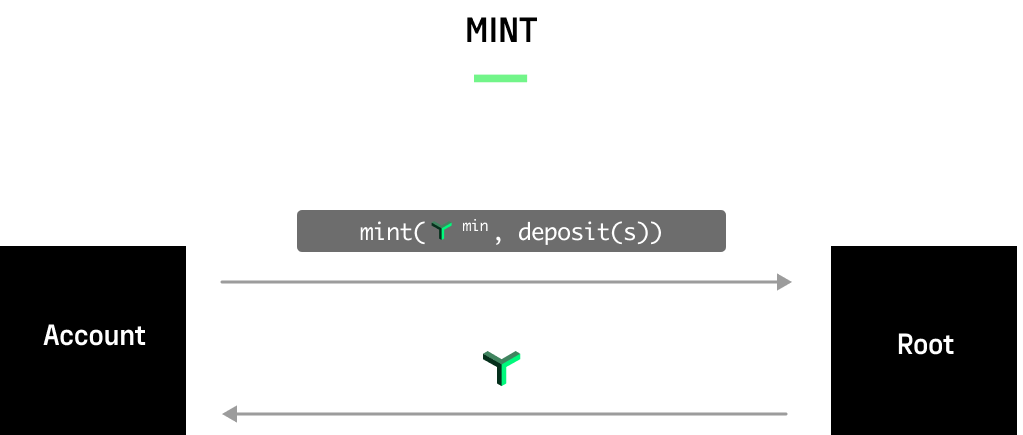
\includegraphics[scale=1]{Figure1}}
    \caption{Mint}
    \label{fig 1}
\end{figure}

\newpage
\subsection{Redeem}
Any account that owns \Root\ can \term{Redeem} them at anytime by calling the \code{redeem} function with (1) the maximum \Root\ to \term{Redeem} ($\Root^{\text{max}}$), such that $\Root^{\text{max}} \in \{j \times 10^{-18} \mid j \in \mathbb{N}\}$, and (2) a list of Beanstalk \term{Silo} \term{Deposits} currently owned by Root. The \Root\ necessary to \term{Redeem} a list of \term{Silo} \term{Deposits} ($\Root^{-}$), such that $\Root^{-} \in \{j \times 10^{-18} \mid j \in \mathbb{Z}\}$, is the minimum of (1) $\Root^{\text{max}}$ and (2) the maximum of the percentage change in the BDV, \term{Stalk} and \term{Seeds} of Root as a result of the \term{Redemption}. 

Therefore, we define $\Root^{-}$ for a given $\Root^{\text{max}}$, list of \term{Silo} \term{Deposits} with $\Sigma l$, $\Sigma k$ and $\Sigma c$, $L$, $K$, $C$ and $\rho$ as:
$$\Root^{-} = \text{min}\left(\Root^{\text{max}}, \text{max}\left(\frac{\Sigma l}{L},\ \frac{\Sigma k}{K},\ \frac{\Sigma c}{C}\right) \times \rho\right)$$

\begin{figure}[h!]
    \centering
    \hbox{\hspace{6em} 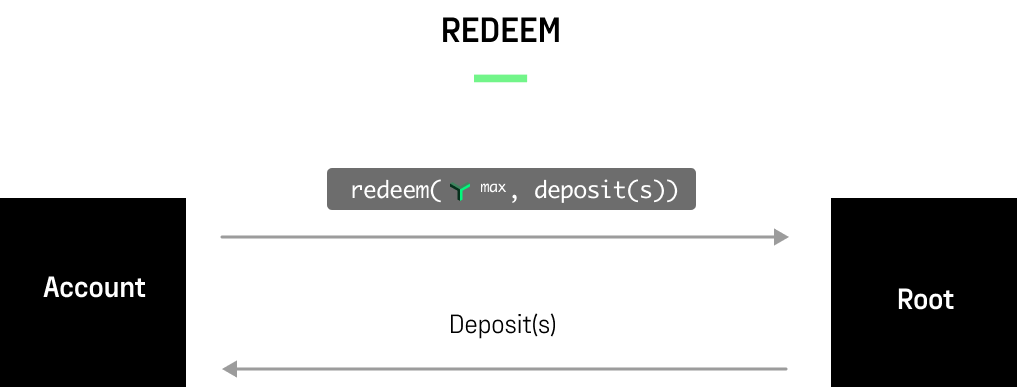
\includegraphics[scale=1]{Figure2}}
    % \hbox{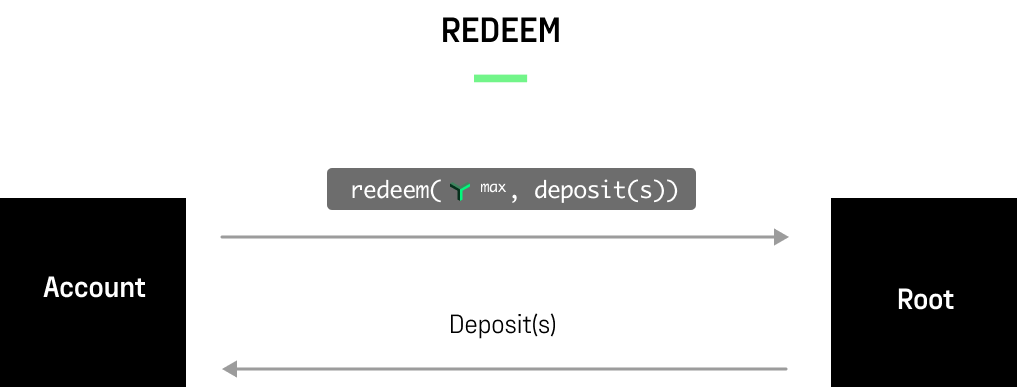
\includegraphics[scale=1.4]{Figure2}}
    \caption{Redeem}
    \label{fig 2}
\end{figure}

\subsection{Earn}
Any account can (1) \term{Mow} all of Root's \term{Grown} \term{Stalk}, (2) \term{Plant} the \term{Seeds} associated with Root's \term{Earned} \Bean and (3) \term{Deposit} Root's \term{Earned} \Bean\ in the current \term{Season}, at anytime by calling the \code{earn} function. This is the only instance the Stalk or Seed per BDV ratios of Root may decrease. 

\begin{figure}[h!]
    \centering
    \hbox{\hspace{1mm} 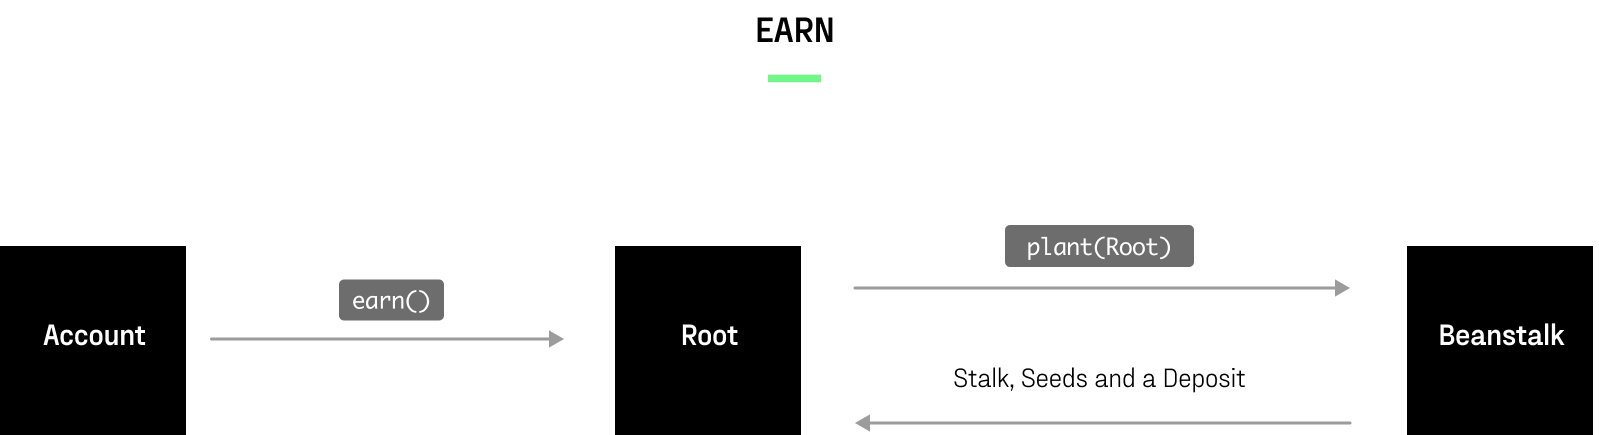
\includegraphics[scale=0.8]{Figure3}}
    \caption{Earn}
    \label{fig 3}
\end{figure}

\newpage
\subsection{Mow}
Any account can \term{Mow} Root's \term{Grown} \term{Stalk} at anytime by calling the \code{mow} function on behalf of Root directly to Beanstalk.

\begin{figure}[h!]
    \centering
    \hbox{\hspace{1mm} 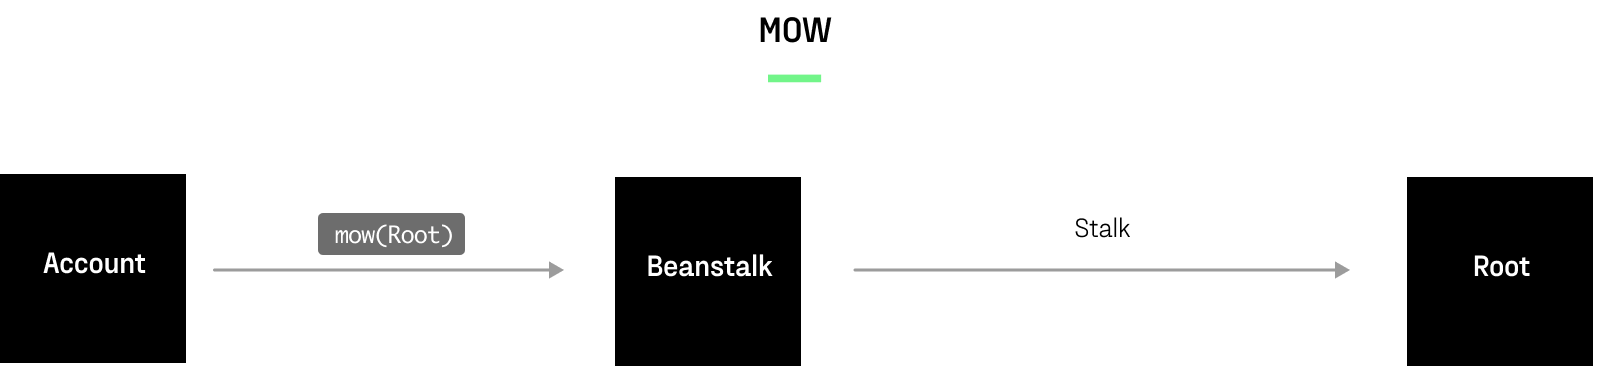
\includegraphics[scale=0.8]{Figure4}}
    \caption{Mow}
    \label{fig 4}
\end{figure}

\subsection{Update BDV}
Any account can update the BDV of one or multiple of Root's \term{Silo} \term{Deposits} at anytime by calling the \code{updateBdv} or \code{updateBdvs} functions, respectively. 

\begin{figure}[h!]
    \centering
    % \hspace{-2cm}
    \hbox{\hspace{1mm} 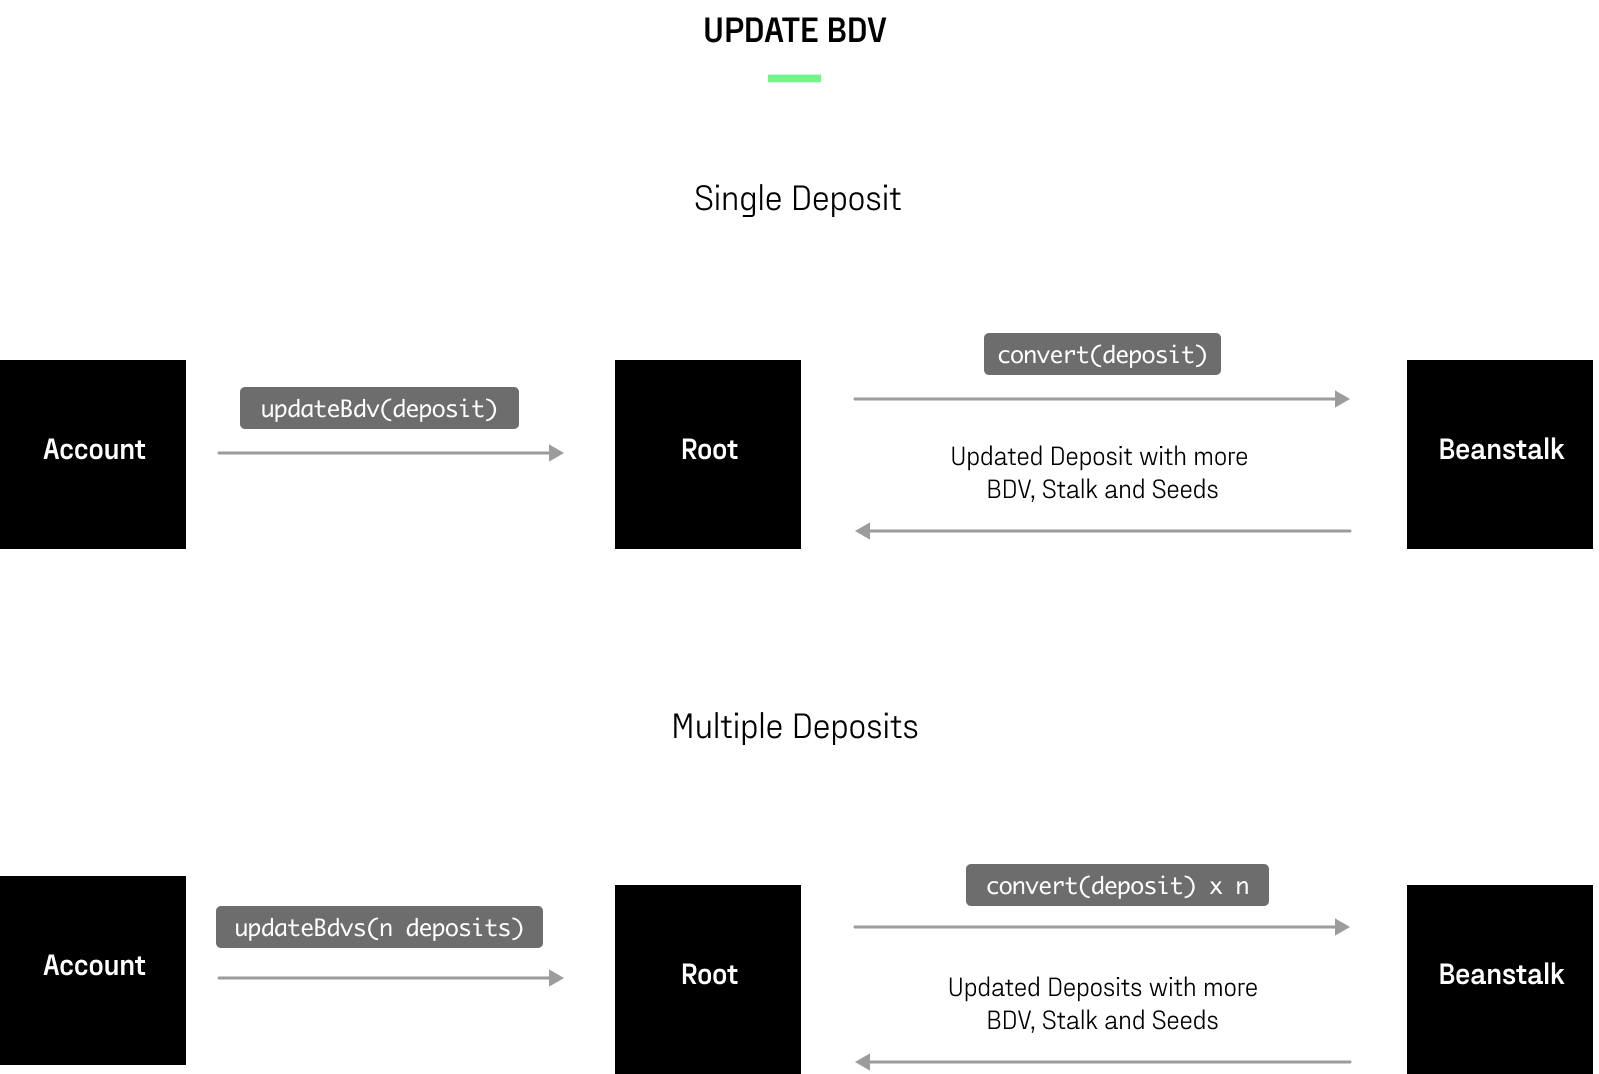
\includegraphics[scale=0.8]{Figure5}}
    \caption{Update BDV}
    \label{fig 6}
\end{figure}

\newpage
\section{Governance}
Root is an upgradable contract. Root's \term{Stalk} ownership gives Root a vote in Beanstalk governance. 

In theory, Root governance should balance (1) ensuring sufficient time for all \Root\ owners to consider a \term{Root Improvement Proposal} (\term{RIP}) and cast their votes or exit the system, with (2) the abilities to be quickly upgraded in cases of emergency and participate in Beanstalk governance. 

In practice, the owner of Root has the exclusive and unilateral ability to commit \term{RIPs}, and vote in Beanstalk governance, at anytime. The owner of each implementation of Root enforces a governance mechanism.

A RIP has 2 inputs: (1) a new contract address and (2) an optional function call.

\section{Economics}
\Root\ owners share all value earned by Root pro rata across all \Root. The pro rata distribution creates a zero-fee shared collective farming option for passive Beanstalk \term{Silo} \term{Depositors} that (1) maximizes Beanstalk-native yield and (2) generates additional yield without creating significant risks to Beanstalk or Root.

The \term{Stalk} and \term{Seeds} owned by Root increase each time an account successfully calls the \code{earn} function. The \term{Stalk} owned by Root increases each time an account successfully calls the \code{mow} function. The BDV, \term{Stalk} and \term{Seeds} owned by Root, and \term{Redeemable} per \Root, increase each time an account successfully calls the \code{updateBdv} or \code{updateBdvs} functions. 

Each time an account \term{Mints} or \term{Redeems} \Root, unless they do so such that the percentage change in the BDV, \term{Stalk} and \term{Seeds} of Root are identical (\term{i.e.}, $\frac{\Sigma l}{L} = \frac{\Sigma k}{K} = \frac{\Sigma c}{C}$), there is some excess BDV, \term{Stalk} or \term{Seeds} that is paid to Root.

\term{Conversions} of Beanstalk \term{Silo} \term{Deposits} within Root are permitted only to increase the BDV of \term{Silo} \term{Deposits}, which prevents manipulation of Beanstalk and Root through price manipulation of Beans.

All non-Beanstalk yield paid to Root is held by Root.

\newpage
\section{Risk}
There are numerous risks associated with Root. This is not an exhaustive list.

The Root code base is novel and has not been tested in the “real world” prior to the initial Root deployment. The open source nature of Root means that others can take advantage of any bugs, flaws or deficiencies in Root and launch identical or very similar Beanstalk fungible \term{Silo} \term{Deposit} wrapper token implementations. 

Root is deployed on the Ethereum network. The security of the Ethereum network is assumed. 

Root is dependent on Beanstalk, and therefore inherits all of the risks associated with Beanstalk. The security of Beanstalk is assumed. For an exhaustive list, consult the Beanstalk Whitepaper\fref{bean.money/beanstalk.pdf\#section.12} and Beanstalk DAO Disclosures.\fref{bean.money/disclosures}

The potential friction to \term{Mint} \Root\ due to the \term{Stalk} or \term{Seed} per \Root\ ratios can make doing so unattractive, thereby limiting supply.

The permissionless and pro rata nature of Root makes it impossible to regulate the ownership distribution of \Root. 

The owner of Root is potentially vulnerable to compromise. 

\section{Future Work}
Root is a work in progress. The following are potential improvements that can be incorporated into Root as one or more \term{RIPs}, or via one or more forks:

\begin{itemize}
    \item A gas-efficient method can be implemented to allow \Root\ owners to permissionlessly claim non-Beanstalk-native yield Root earns, pro rata. 
    \item The governance process around \term{RSPs} can be further refined to maximize Root's ability to participate in non-Root governance.
    \item A system that facilitates \term{Converts} within Root, beyond solely increasing the BDV of \term{Silo} \term{Deposits}, without creating the potential for manipulation can be implemented.
    \item Root should vote only the portion of its \term{Stalk} corresponding to the percent of \Root\ that vote for a given \term{BIP} once Beanstalk supports partial votes. 
    \item Root should implement on-chain governance once Beanstalk returns to it. 
\end{itemize}

\newpage
\section{Appendix}
\documentclass[class=article, crop=false]{standalone}
\usepackage[subpreambles=true]{standalone}
\usepackage{import}
\usepackage{amsmath}
\usepackage{enumitem} % Format list spacing 

\begin{document}
\subsection{Implementations}
The following is an incomplete list of implementations of Root.

\subsubsection{0x77700005BEA4DE0A78b956517f099260C2CA9a26}
The Root contract address is 0x77700005BEA4DE0A78b956517f099260C2CA9a26 \newline(\term{i.e.}, \Root\ = 0x77700005BEA4DE0A78b956517f099260C2CA9a26).

\paragraph{Current Parameters}
The following are the current parameters of 0x77700005BEA4DE0A78b956517f099260C2CA9a26:
\begin{itemize}[itemsep=3pt,leftmargin=16pt]
    \item The owner of 0x77700005BEA4DE0A78b956517f099260C2CA9a26 is \newline0xb7774ec5031e1d903152E96BbC1601e5D0D83Ca2 (\term{i.e.}, the \term{Root DAO Multisig});
    \item The address of Beanstalk is 0xC1E088fC1323b20BCBee9bd1B9fC9546db5624C5; and
    \item $\Root^{\text{min}}$ = 0.1\%.
\end{itemize}

\paragraph{Minting Whitelist}
The following ERC-20 Standard tokens are on the Beanstalk \term{Deposit} \term{Whitelist} and \term{Whitelisted} for \term{Minting} \Root:

\begin{itemize}[itemsep=3pt,leftmargin=16pt]
    \item 0xBEA0000029AD1c77D3d5D23Ba2D8893dB9d1Efab (\term{i.e.}, \Bean).
\end{itemize}

\paragraph{Governance}
A robust decentralized governance mechanism must balance the principles of decentralization with resistance to attempted protocol changes, both malicious and ignorant, and the ability to quickly adapt to changing information. 

0x77700005BEA4DE0A78b956517f099260C2CA9a26 is governed by Root DAO. Root DAO governs upgrades to 0x77700005BEA4DE0A78b956517f099260C2CA9a26, the use of \term{Stalk} in Beanstalk governance and the treatment of non-Beanstalk-native yield earned by \newline0x77700005BEA4DE0A78b956517f099260C2CA9a26. Any account that owns \Root\ can participate in Root DAO governance.

\subparagraph{RIPs}

Any account that owns more than $\Root^{\text{RIP}}$, such that $\Root^{\text{RIP}} \in \{j \times 10^{-18} \mid j \in \mathbb{N},\ j \leq 10^{18} \}$, of total outstanding \Root\ can submit a \term{RIP} to the Root DAO Snapshot\fref{snapshot.org/\#/rootsmoney.eth} via the \term{Root DAO Multisig}.

Root DAO only accepts votes in favor of \term{RIPs}. An account's vote for a given \term{RIP} is counted as the minimum of its \Root\ between the beginning and end of the \term{Voting Period}. 

A \term{Voting Period} begins when a vote for a \term{RIP} can be submitted to Snapshot and ends at approximately the beginning of the 169th Beanstalk \term{Season} after it begins, or when the \term{RIP} is committed with a supermajority.

If at the end of the \term{Voting Period}:
\begin{itemize}[midsep]
    \item Less than or equal to half of the total outstanding eligible \Root\ votes in favor of the \term{RIP}, it fails; and
    \item More than half of the total outstanding eligible \Root\ votes in favor of the \term{RIP}, it passes.
\end{itemize}

If at any time before the end of the \term{Voting Period} more than two-thirds of the total outstanding eligible \Root\ votes in favor of the \term{RIP}, it passes and can be committed to the Ethereum blockchain.

\subparagraph{Stalk Use}
In its capacity as a \term{Stalkholder}, 0x77700005BEA4DE0A78b956517f099260C2CA9a26 is entitled to vote on (1) each \term{Beanstalk Improvement Proposal} (\term{BIP}) and (2) other, non-\term{BIP}, governance processes, and may be entitled to non-Beanstalk-native yields.

Any \Root\ owner can submit a \term{Root Stalk Proposal} (\term{RSP}) to the \term{RSP} Snapshot\fref{snapshot.org/\#/rootstalkproposals.eth} to determine how Root should use its \term{Stalk} in each governance process, and distribute yields, if ever. \term{RSPs} follow the same structure as \term{RIPs}, except that the length of the \term{Voting Period} can be reasonably shortened to ensure the will of Root DAO can be reflected in the governance process.

Any \term{Beanstalk Improvement Proposal} (\term{BIP}) will automatically qualify to be proposed to Root DAO as an \term{RSP}.

The \term{Root DAO Multisig} will participate on each governance process as determined by the \term{RSP}.

\subparagraph{Root DAO Multisig}
The \term{Root DAO Multisig} is a 4-of-7 Safe\fref{app.safe.global/eth:0xb7774ec5031e1d903152E96BbC1601e5D0D83Ca2} multisig wallet with anonymous signers consisting of community members and contributors to Root and Beanstalk. The \term{Root DAO Multisig} will execute the will of Root DAO. The \term{Root DAO Multisig} will provide sufficient notice of the submission of a \term{RIP}, its contents and the beginning of its \term{Voting Period} before submitting a \term{RIP} to Snapshot, and will repost \term{BIPs} on the \term{RSP} Snapshot as soon as possible after they are posted to the Beanstalk DAO Snapshot.\fref{snapshot.org/\#/beanstalkdao.eth} In the future, we expect \term{RIPs} will implement permissionless governance and revoke these abilities from the \term{Root DAO Multisig}.

Thus, Root creates a robust decentralized governance mechanism.
\end{document} % Initial Parameters

\newpage
\documentclass[class=article, crop=false]{standalone}
\usepackage[subpreambles=true]{standalone}
\usepackage{import}
\usepackage{enumitem} % Format list spacing 

\begin{document}

\subsection{Glossary}
The following conventions are adopted from the Beanstalk Whitepaper and used throughout this Whitepaper:
\begin{itemize}
    \item Lower case Latin letters are unique values;
    \item Upper case Latin letters are totals or rates; and
    \item Superscripts are modifiers.
\end{itemize}

The following variables and terms are used throughout this paper:
\begin{itemize}[topsep=0pt, itemsep=3pt,leftmargin=16pt]
    \item[] \Bean\ - Bean;
    \item[] BDV - Bean-denominated-value;
    \item[] Beanstalk - The issuer of \Bean\ and \term{Silo} \term{Deposits}; 
    \item[] \term{Beanstalk Improvement Proposal} - A Beanstalk governance proposal;
    \item[] \term{BIP} - A \term{Beanstalk Improvement Proposal};
    \item[] $\Sigma c$ - The cumulative \term{Seeds} for a given list of \term{Silo} \term{Deposits};
    \item[] $C$ - Root's total \term{Seeds};
    \item[] \term{Convert} - Turn one or more \term{Silo} \term{Deposits} into another, within the \term{Silo};
    \item[] DAO - Decentralized autonomous organization;
    \item[] DeFi - Decentralized finance;
    \item[] \term{Deposit} - An asset in the \term{Silo};
    \item[] \term{Deposit} \term{Whitelist} - The Beanstalk whitelist that permissions which tokens can be \term{Deposited} into the \term{Silo};
    \item[] \term{Depositors} - An account that has \term{Deposited} assets into the \term{Silo};
    \item[] \term{Earned} \Bean\ - Beans paid to a \term{Stalkholder} after the last \term{Season} the \term{Stalkholder} called the \code{plant()} function;
    \item[] \term{Grown} \term{Stalk} - \term{Stalk} that has \term{Grown} from \term{Seeds} but not yet \term{Mown};
    \item[] $\Sigma k$ - The cumulative \term{Stalk} for a given list of \term{Silo} \term{Deposits};
    \item[] $K$ - Root's total \term{Stalk};
    \item[] $\Sigma l$ - The cumulative BDV for a given list of \term{Silo} \term{Deposits};
    \item[] $L$ - Root's total BDV;
    \item[] LP - Liquidity pool;
    \item[] \term{Mint} - Turn one or more Beanstalk \term{Silo} \term{Deposits} into \Root;
    \item[] \term{Minting} \term{Whitelist} - The Root whitelist that permissions using Beanstalk \term{Silo} \term{Deposits} to \term{Mint} \Root;
    \item[] \term{Mow} - Turn \term{Grown} \term{Stalk} into \term{Stalk};
    \item[] \term{Plant} - Turn \term{Plantable} \term{Seeds} associated with \term{Earned} \Bean\ into \term{Seeds} by \term{Depositing} the \term{Earned} \Bean\ in the current \term{Season};
    \item[] \term{Redeem} - Turn \Root\ into one or more Beanstalk \term{Silo} \term{Deposits};
    \item[] \term{RIP} - A \term{Root Improvement Proposal};
    \item[] \term{Root Improvement Proposal} - A Root governance proposal;
    \item[] \term{Root Stalk Proposal} - A Root governance proposal to determine how Root should use its \term{Stalk} in a given instance unrelated to \term{RIPs};
    \item[] \term{RSP} - A \term{Root Stalk Proposal};
    \item[] \term{Root DAO Multisig} - The owner of the Root contract;
    \item[] \term{$\rho$} - The total \Root\ supply;
    \item[] \Root\ - Roots; Root's ERC 20 Standard token;
    \item[] $\Root^{\text{max}}$ - The maximum \Root\ to \term{Redeem};
    \item[] $\Root^{\text{min}}$ - The minimum \Root\ to \term{Mint};
    \item[] $\Root^{\text{RIP}}$ - The percentage of \Root\ ownership necessary to submit a \term{RIP};
    \item[] \term{Season} - Beanstalk-native discrete time;
    \item[] \term{Seed} - A Beanstalk-native asset that \term{Grows} $1 \times 10^{-4}$ \term{Stalk} each \term{Season};
    \item[] \term{Silo} - The Beanstalk DAO;
    \item[] \term{Stalk} - The Beanstalk-native governance asset;
    \item[] \term{Stalkholder} - An owner of \term{Stalk}; a Beanstalk DAO member; and
    \item[] \term{Voting Period} - The period of time \Root\ owners can vote on a \term{RIP} or \term{RSP}.
\end{itemize}
\end{document} % Glossary

\newpage
\documentclass[class=article, crop=false]{standalone}
\usepackage[subpreambles=true]{standalone}
\usepackage{import}
\usepackage{enumitem} % Format list spacing 

\begin{document}

\subsection{Whitepaper Version History}
The following is a complete version history of this Whitepaper. Unless otherwise noted, references within this Whitepaper Version History are not updated to reflect later changes.

\begin{itemize}[topsep=0pt, itemsep=3pt,leftmargin=16pt]
    \item \href{https://github.com/RootToken/Root-Whitepaper/blob/master/version-history/root1_0_0.pdf}{1.0.0} (November 16, 2022)
    \begin{itemize}
        \item Original Whitepaper.
    \end{itemize}
    \item \href{https://github.com/RootToken/Root-Whitepaper/blob/master/version-history/root1_0_1.pdf}{1.0.1} (November 28, 2022)
    \begin{itemize}
        \item Updated citations 2, 4 and 6 with the new URL for the Beanstalk Whitepaper.
        \item Capitalized Beanstalk Whitepaper in \hyperlink{section.6}{Section 6}.
        \item Updated citation 7 with the new URL for the Beanstalk DAO Disclosures.
        \item Changed Gnosis to Safe in \hyperlink{subparagraph.8.1.1.3.3}{Section 8.1.1.3.3}.
        \item Updated citation 10 with the correct URL and address for the \term{Root DAO Multisig}.
        \item Changed paper to Whitepaper in the intro to the \hyperlink{subsection.8.2}{Glossary}.
    \end{itemize}
    \item \href{https://github.com/RootToken/Root-Whitepaper/blob/master/version-history/root1_0_2.pdf}{1.0.2} (December 2, 2022)
    \begin{itemize}
        \item Updated the entire paper to remove all subscripts, which were denoting time, from the whitepaper, because they are no longer necessary.
        \item Corrected the domain of $\Root^{+}$.
        \item Updated the equations for $\Root^{+}$ and $\Root^{-}$.
        \item Added $C$, $K$, $L$ and $\rho$ to the \hyperlink{subsection.8.3}{Glossary}. 
        \item Removed $C_{<\Game}$, $C_{\Game>}$, $K_{<\Game}$, $K_{\Game>}$, $L_{<\Game}$ and $L_{\Game>}$ from the \hyperlink{subsection.8.2}{Glossary}. 
    \end{itemize}
    \item \href{https://github.com/RootToken/Root-Whitepaper/blob/master/version-history/root1_0_3.pdf}{1.0.3} (January 24, 2023)
    \begin{itemize}
        \item Corrected the calculation for \Root\ necessary to \term{Redeem} a list of \term{Silo} \term{Deposits}.
        \item Corrected the Whitepaper Version 1.0.2 number in the \hyperlink{subsection.8.3}{Whitepaper Version History}. 
    \end{itemize}
\end{itemize}
\end{document} % Whitepaper Version History

\end{document}